\documentclass[aps,pre,twocolumn,letterpaper,floatfix]{revtex4}
\usepackage{graphicx} 
\usepackage{amsmath,amssymb,amsfonts} 
\usepackage{mathtools}
\usepackage{pdfpages}
\usepackage{afterpage}
\usepackage[hidelinks]{hyperref} 
\usepackage{epstopdf}
\usepackage{todo}
\begin{document}

\title{Atomify - a live LAMMPS visualizer}
\author{Anders Hafreager$^1$}
\author{Svenn-Arne Dragly$^{1}$} 
\author{Anders Malthe-S\o renssen$^1$}
\affiliation{$^1$Department of Physics - University of Oslo\\Sem S{\ae}lands vei 24, NO-0316, Oslo, Norway }
\date{\today} 

%%%%%%%%%%%%%%%%%%%%%%%%%%%%%%%%%%%%%%%%%%%%%%%%%%%%%%%%%%%%%
%%%%%%%%%%%%%%%%%%%%%%%%%%%%%%%%%%%%%%%%%%%%%%%%%%%%%%%%%%%%%

\begin{abstract}
%
The typical workflow when developing LAMMPS scripts includes working with
several programs.
A text editor is needed to modify the scripts,
the terminal to run the simulation, and programs like VMD or Ovito to visualize
the system over time.
If physical quantities are computed, the data is often plotted with MATLAB or
Python, where additional scripts must be used.
This is a tedious process, especially for teaching purposes and for people who
are new to LAMMPS.
We here introduce Atomify;
a high performance live visualizer for LAMMPS simulations,
with stunning graphics able to simulate and render more than 250000 atoms with
excellent frame rate on modern hardware.
Atomify supports OpenMP acceleration, live plotting of LAMMPS variables and
computes, and an easy-to-use code editor in one single program.
Direct access to the powerful machinery already built into LAMMPS allows easy
access to advanced physical quantities.
Atomify is open-source software (GPL) written in C++ using the Qt framework.
%
\end{abstract} 
 
\maketitle

\section{Introduction}
%
Molecular dynamics (MD) is a common technique for simulating the motion of atoms
and molecules in a broad range of fields.
% TODO does MD also include larger particles?
% TODO which fields?
Over the years, increasingly sophisticated methods have been developed.
% TODO what methods?
With the large number of force fields, advanced techniques and GPU acceleration,
implementing a good molecular dynamics simulation is a challenging task.
There are many software packages for molecular dynamics modelling
available
\footnote{See \url{https://en.wikipedia.org/wiki/Comparison_of_software_for_molecular_mechanics_modeling}.}
Some packages, such as LAMMPS\cite{Plimpton1995Fast}, GROMACS\cite{Pronk2013}
and NAMD\cite{Phillips2005Scalable} have been developed for more than two decades 
and contain more than one million lines of code each.

The work in this paper is focused on LAMMPS.
Although the software is well-documented and enables the user to perform
advanced simulations, it can be demanding to learn how to use it well.
A LAMMPS simulation is performed by a series of commands which are executed one by
one.
Physical quantities such as energy, temperature and stress can be measured by
adding \textit{computes}.
The time evolution of these quantities can in turn be saved to file for plotting
and further analysis.
Particle trajectories can be saved to a file and visualized by tools such as
VMD\cite{Humphrey1996Vmd} or OVITO\cite{Stukowski2009Visualization}.
The lack of an intuitive GUI and visualization \footnote{which are listed in the
non-features list on the web page:
\url{http://lammps.sandia.gov/non_features.html}} makes the workflow somewhat
complicated.

Atomify solves combines script editing, simulation,
visualization, and analysis in one single software application.
It uses LAMMPS as a library and synchronizes after each timestep,
copying the relevant information from LAMMPS to the graphics processing unit
(GPU) for visualization and data plotting.
The visualization is optimized for high performance by raytracing on billboards.
This allows visualization of millions of atoms with good framerate on desktop
computers. Atomify is designed with simplicity as main goal.

TODO: Write about existing GUI software such as Materials Studio and MacroModel \\

A simplified version of Atomify is made available for mobile platforms (Android
and iOS).
This version of Atomify provides access to some of the examples and is intended
for exploration of molecular dynamics simulations by students.
It also works as a demonstration of the visualization capabilities of the
desktop version of the software.
The authors are optimistic that teachers can use the visualizations provided by
Atomify to explain microscopic interactions underlying concepts in topics such
as thermodynamics, geophysics, and biology.

\begin{figure}
	\centering
	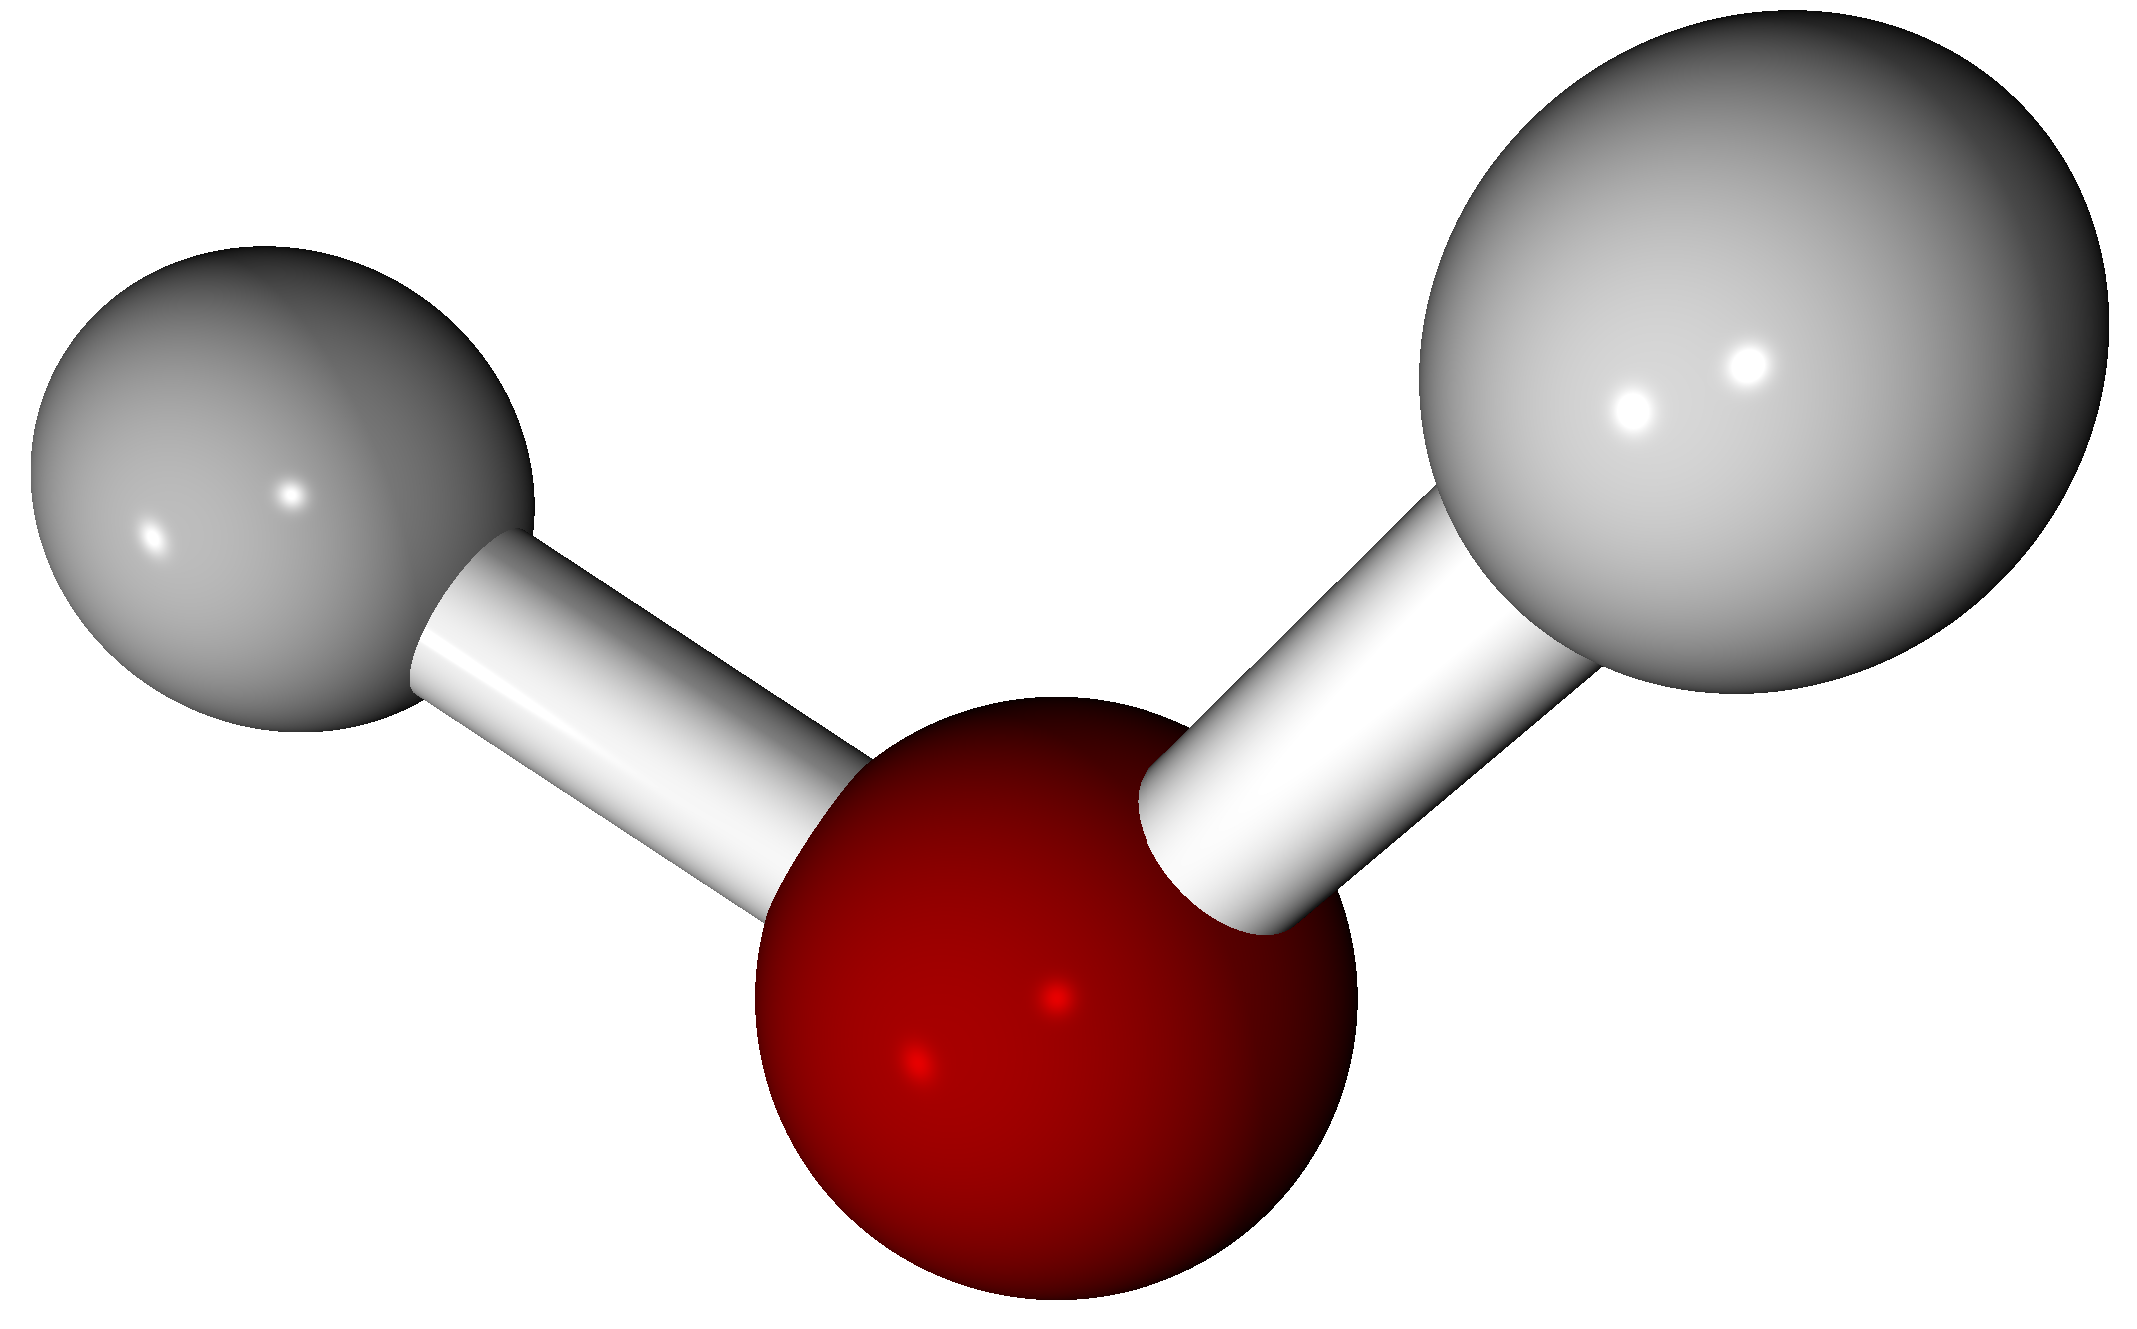
\includegraphics[width=0.5\textwidth]{final_billboard.png}
	\caption{Oversikt over GUI}
	\label{fig:gui}
\end{figure}

\section{Features}

The main features of Atomify are script editing,
live visualization, and live plotting of computed quantities.
These will be described in detail in the following paragraphs.
In addition, Atomify comes packaged with multiple examples,
many of which have been made by members of the LAMMPS community.
These examples are easily explored within Atomify.

\begin{figure}
	\centering
	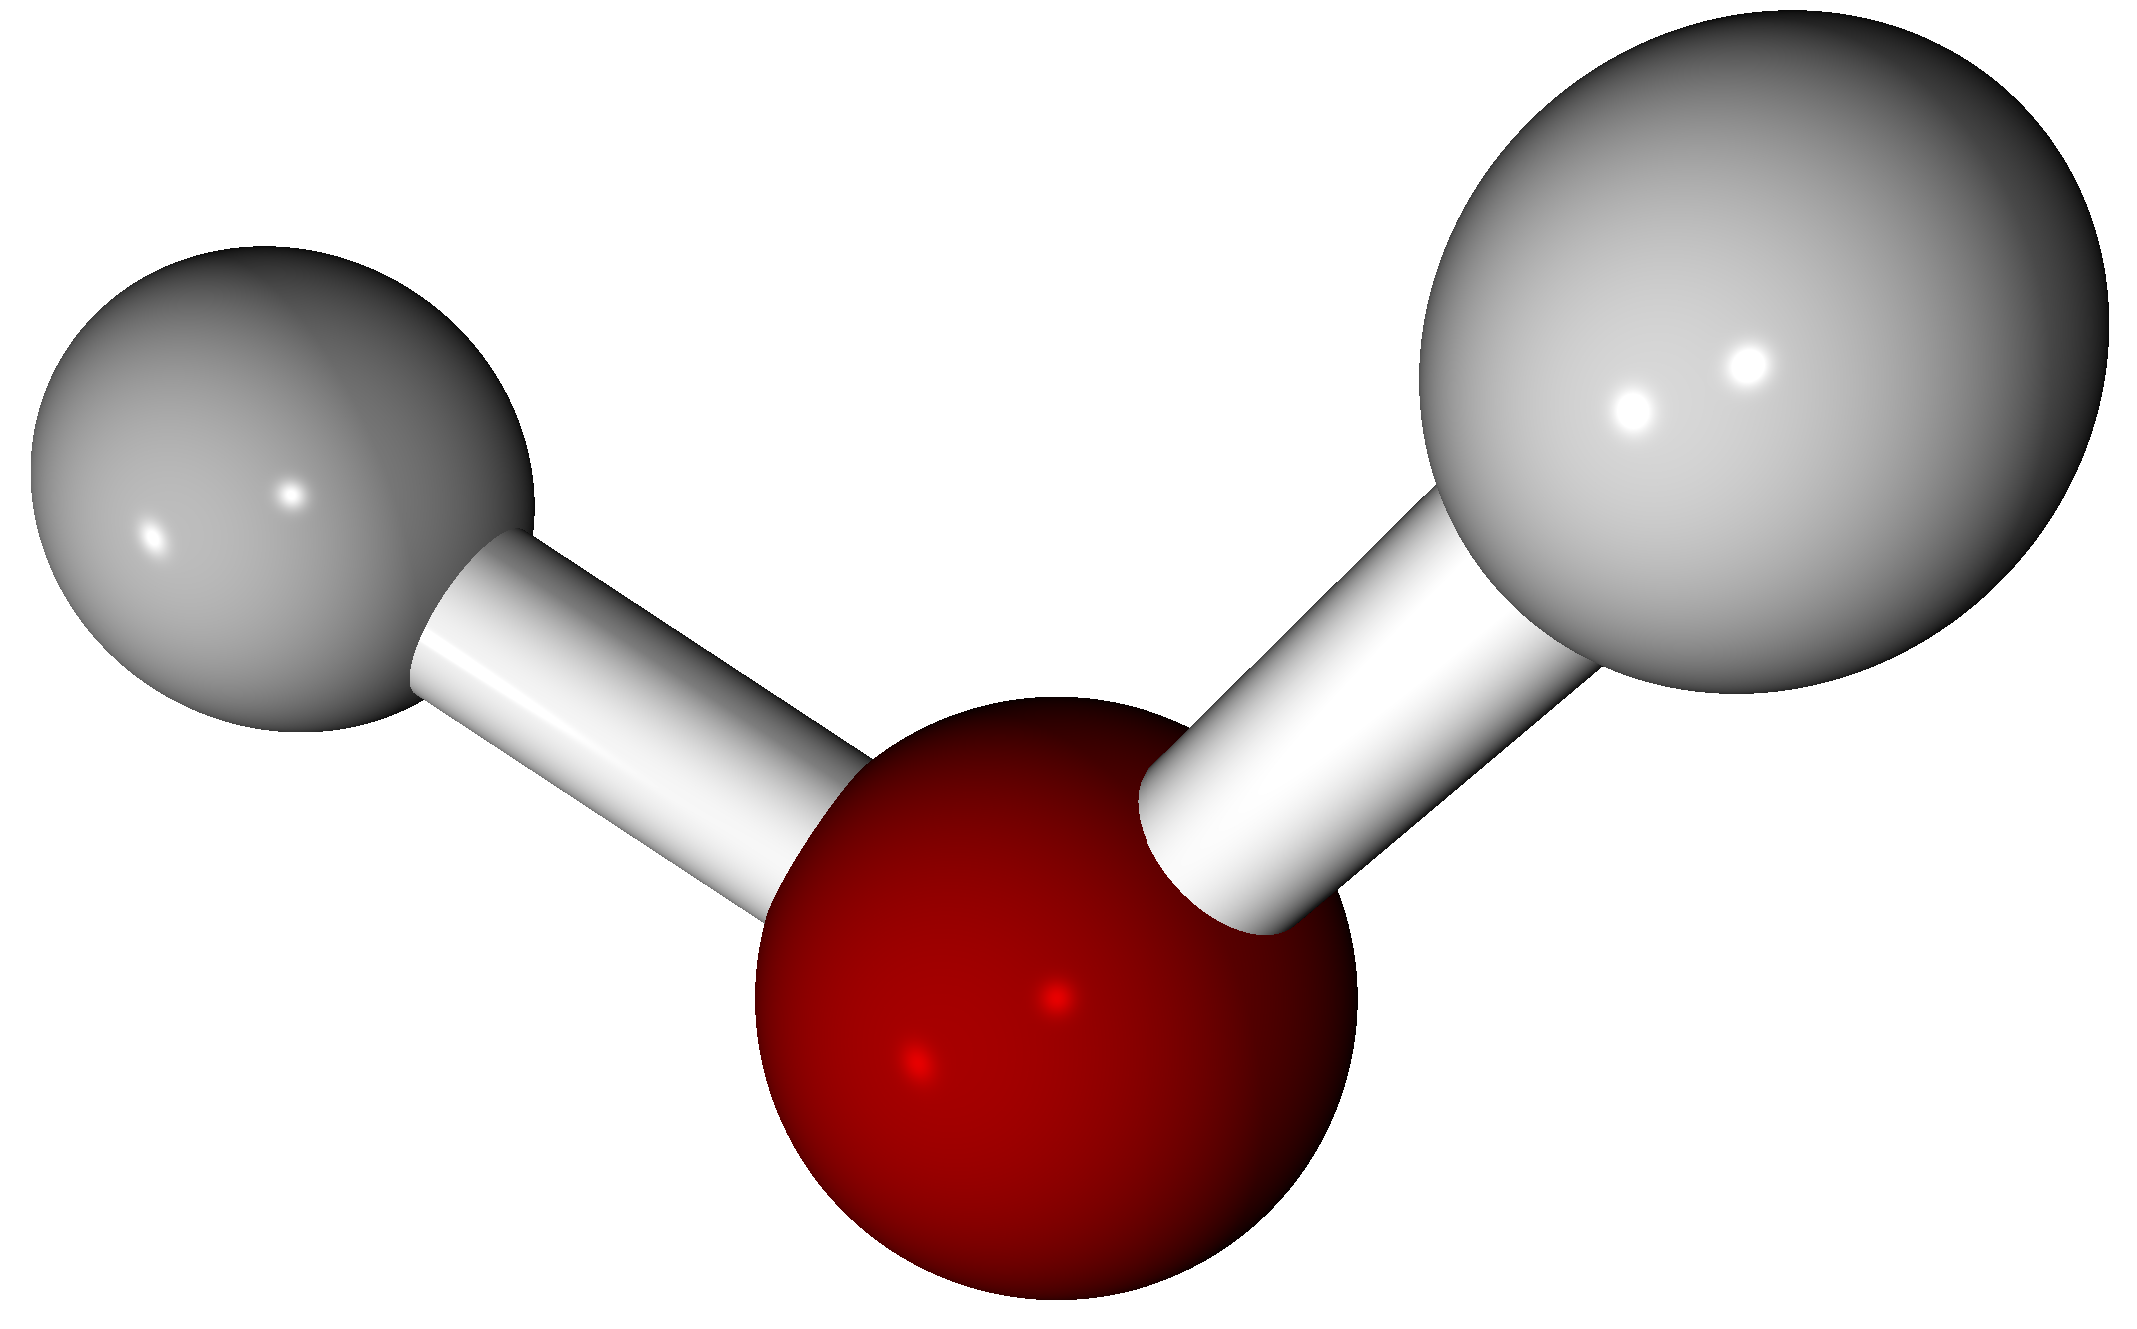
\includegraphics[width=0.5\textwidth]{final_billboard.png}
	\caption{Workflow}
	\label{fig:gui}
\end{figure}

% TODO list other, smaller features that are not in the following subsections or create more subsections for bigger features

\subsection{Script editor}
Atomify provides a lightweight script editor with syntax highlighting and line
numbers.
% TODO add built-in help and autocompletion to Atomify and mention here
Multiple files can be open at the same time and persist across working sessions.
The script can easily be restarted by clicking the button in the GUI or using
the default shortcut (Ctrl+R in Windows and Linux or Cmd+R in macOS).
Any changes made to the script are immediately visualized in the simulation.

\subsection{Visualization}
TODO: Color atoms based on property \\

\subsection{Dashboard}
TODO: Highlight groups/regions \\
TODO: Show/hide groups/regions \\
TODO: Rendering parameters \\
TODO: Atomify commands \\
TODO: Rendering parameters \\
TODO: Plot compute/variable/fix \\

\subsection{Live plotting}
TODO: Histogram over per atom quantities \\
TODO: Time evolution of quantity \\
TODO: 2d ave/chunk binning \\

In LAMMPS, computes are physical quantities calculated based on the running
simulation, such as energy, temperature, and stress.
% TODO better word for measures?
These are typically macroscopic measures derived from the microscopic
interactions between the atoms.

Atomify provides live visualization of the compute values using various plotting
techniques.
For instance, the temperature of the simulated system can be plotted as a
function of time as seen in figure TODO.
% TODO add figure

\begin{figure}
	\centering
	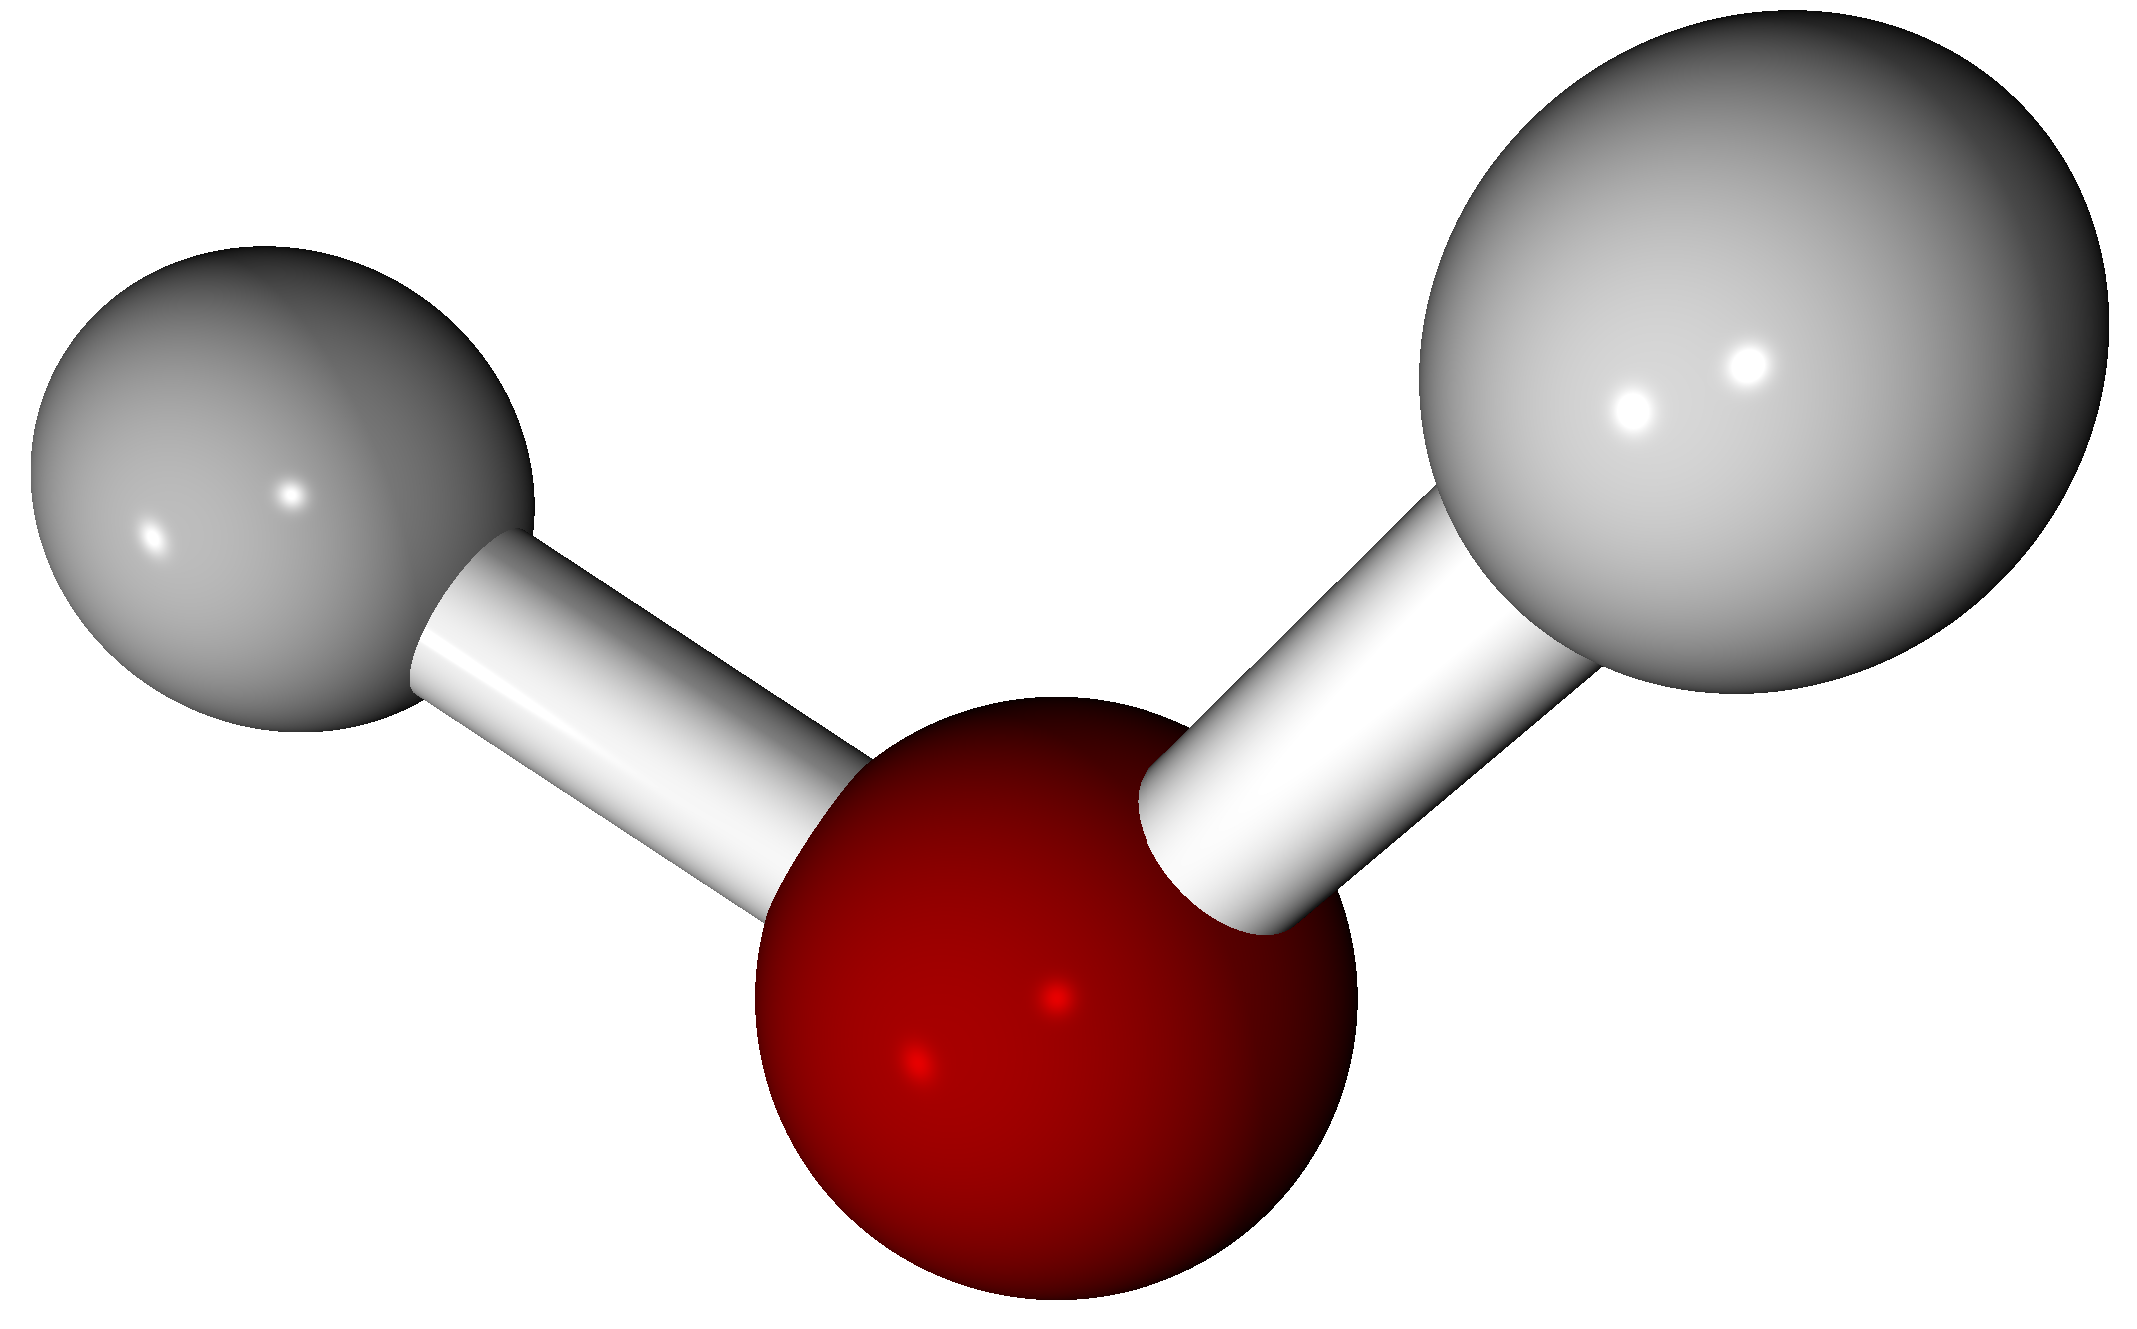
\includegraphics[width=0.5\textwidth]{final_billboard.png}
	\caption{Features}
	\label{fig:gui}
\end{figure}

\section{Implementation}

Atomify is built upon Qt.
All GUI is defined in QML whereas the backend of the program communicating with
LAMMPS is written in C++.
High-performance visualization is achieved by implementing billboards in Qt3D.
Simply put, Atomify runs an instance of a LAMMPS object enabling the user to
visualize the current state of LAMMPS and interact with LAMMPS while the
simulation is running. 

\begin{figure}
	\centering
	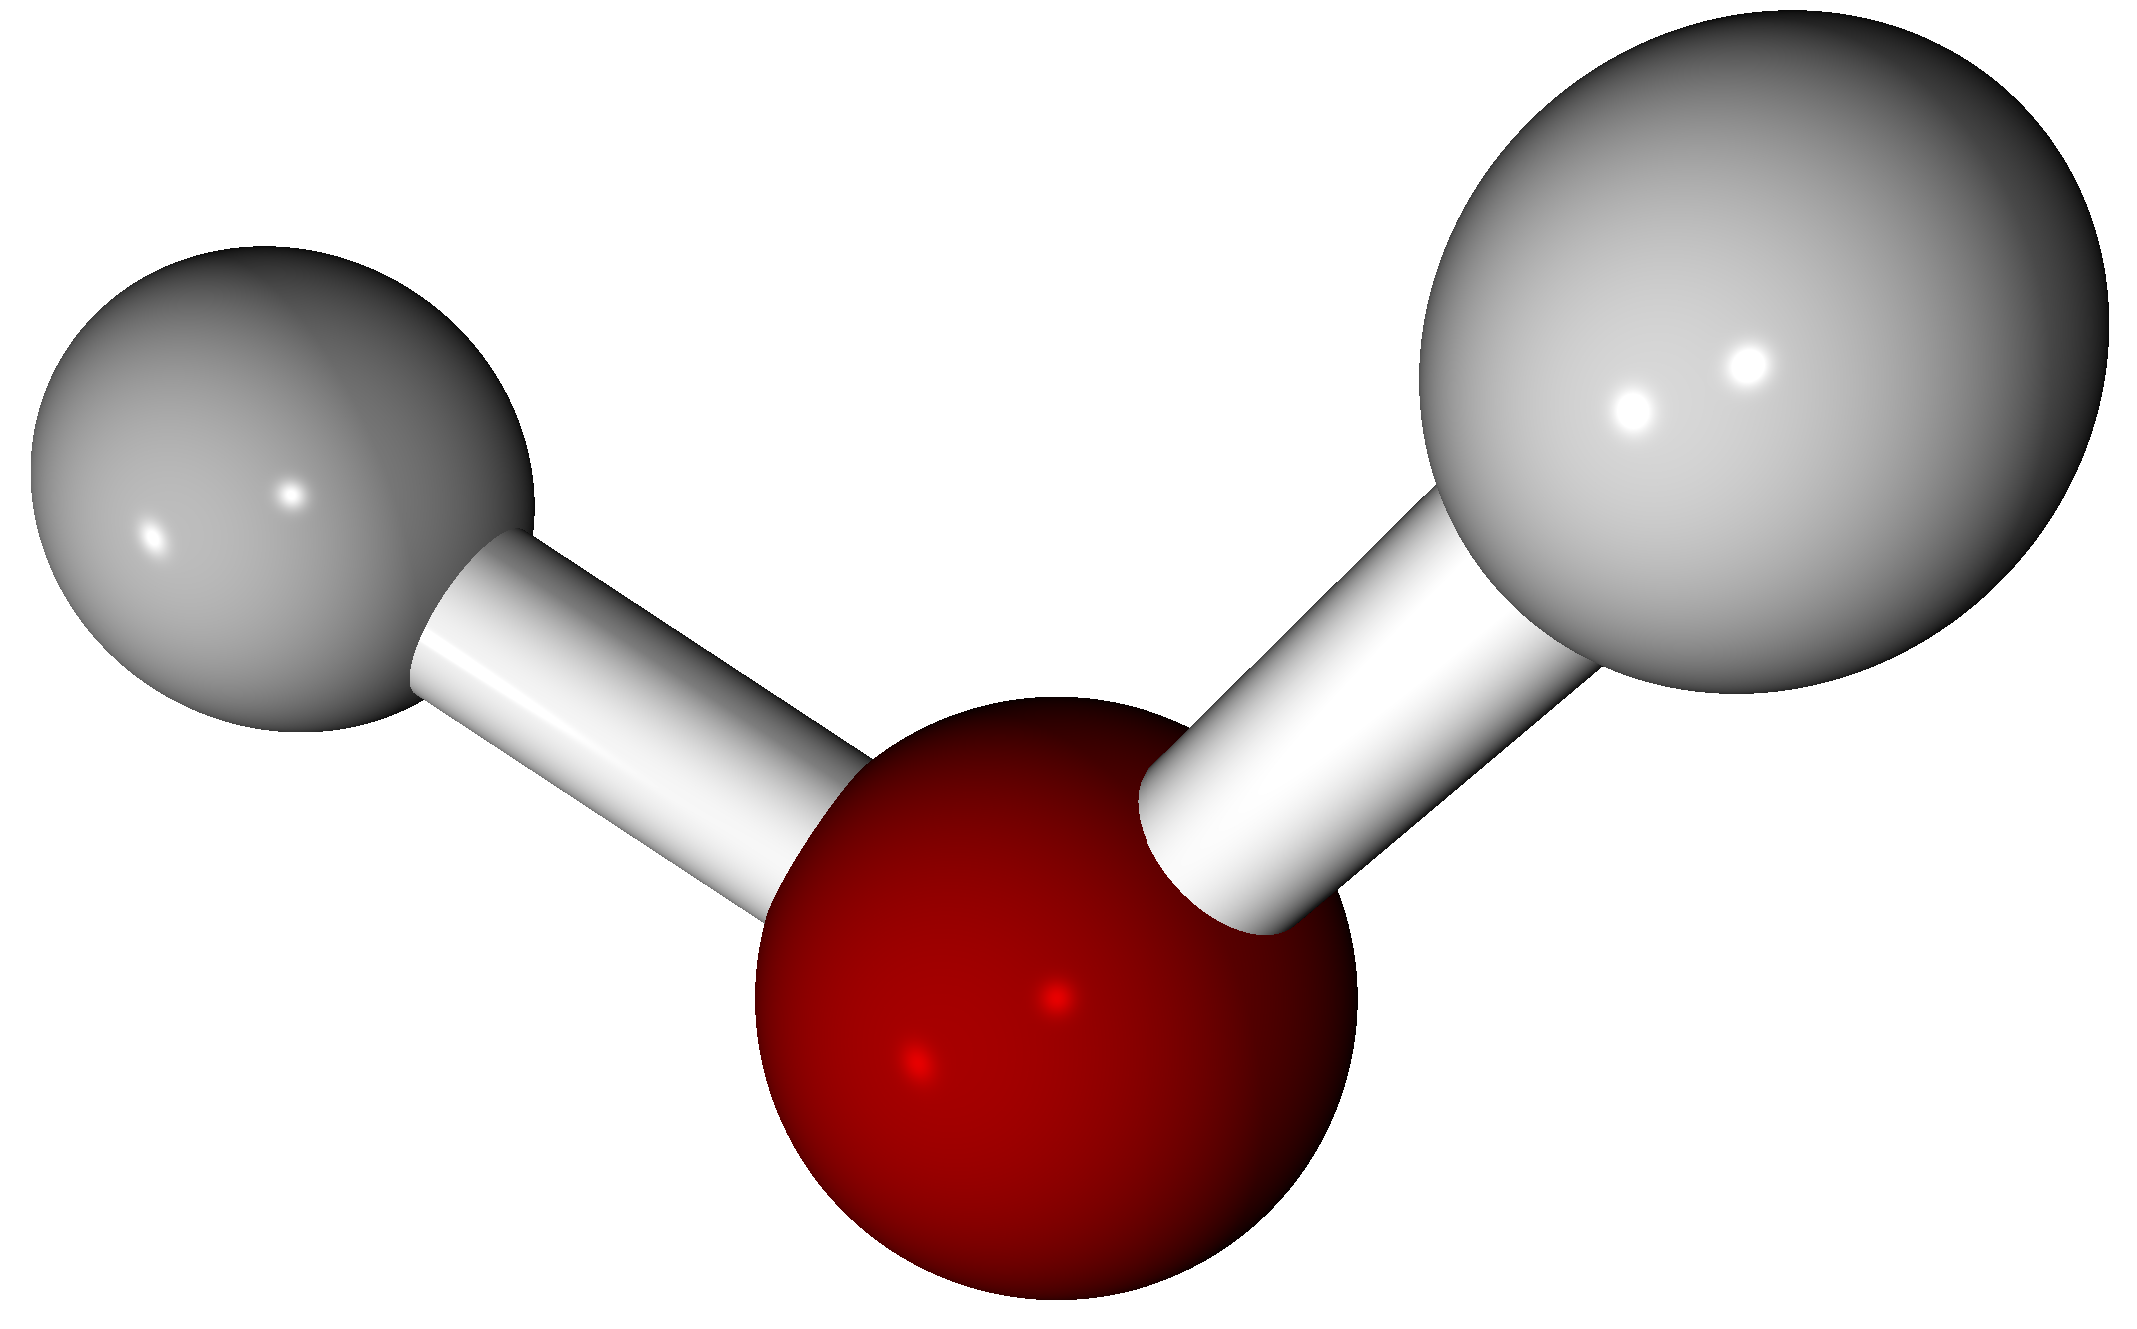
\includegraphics[width=0.5\textwidth]{final_billboard.png}
	\caption{Data pipeline (lammps -> atomify)}
	\label{fig:gui}
\end{figure}

\subsection{Communicating with LAMMPS}

LAMMPS can be compiled as a library with most of its contents being accessable
through either the library interface or public variables in all classes.
LAMMPS provides a C++ API that can be used to access parts of the internal data
in the simulation as well as for issuing commands to LAMMPS.
Further, direct access to raw data in LAMMPS is available through the individual
C++ classes.

\subsection{Live plotting}

Live plotting is implemented using Qt Charts and Qt Data Visualization,
which are part of the Qt framework.
The data is extracted using LAMMPS' C++ API and converted to Qt datatypes before
visualization.

\subsection{Data pipeline}

When rendering one often wants to modify the data
from LAMMPS before it is visualized.
Examples are periodic images of the simulation,
slicing and coloring.
We have been inspired by the pipeline used in Ovito where the data flows through
several \textit{modifiers}, each modifying the visualization data before the
data is converted to a format for the GPU.

\section{Rendering techniques}

Simulations of atoms are often visualized using spheres as atoms and cylinders.
The spheres represent the atoms while the cylinders represent the bonds between
the atoms.
This way, the molecular structure is easy to understand and interpret.
In many visualization tools, the spheres and cylinders are built up by many
triangles connected so they form the geometrical object of interest.
One problem with this rendering technique is that each sphere needs many,
often hundreds, of triangles in order to look spherical.
A common technique to overcome this problem is to use billboards.
This significantly reduces the number of vertices sent from the CPU to the GPU,
which in turn improves rendering performance.
A sphere may consist of an arbitrary number of vertices,
depending on the level of detail needed.
A billboard will on the other hand consist of only 4 vertices and can be
represented as a point on the CPU which is then expanded on the GPU using shader
programming.
By doing proper shading, the billboards can mimick the spheres and cylinders so
they look realistic, see Figure \ref{fig:final_billboards}.

\begin{figure}
	\centering
	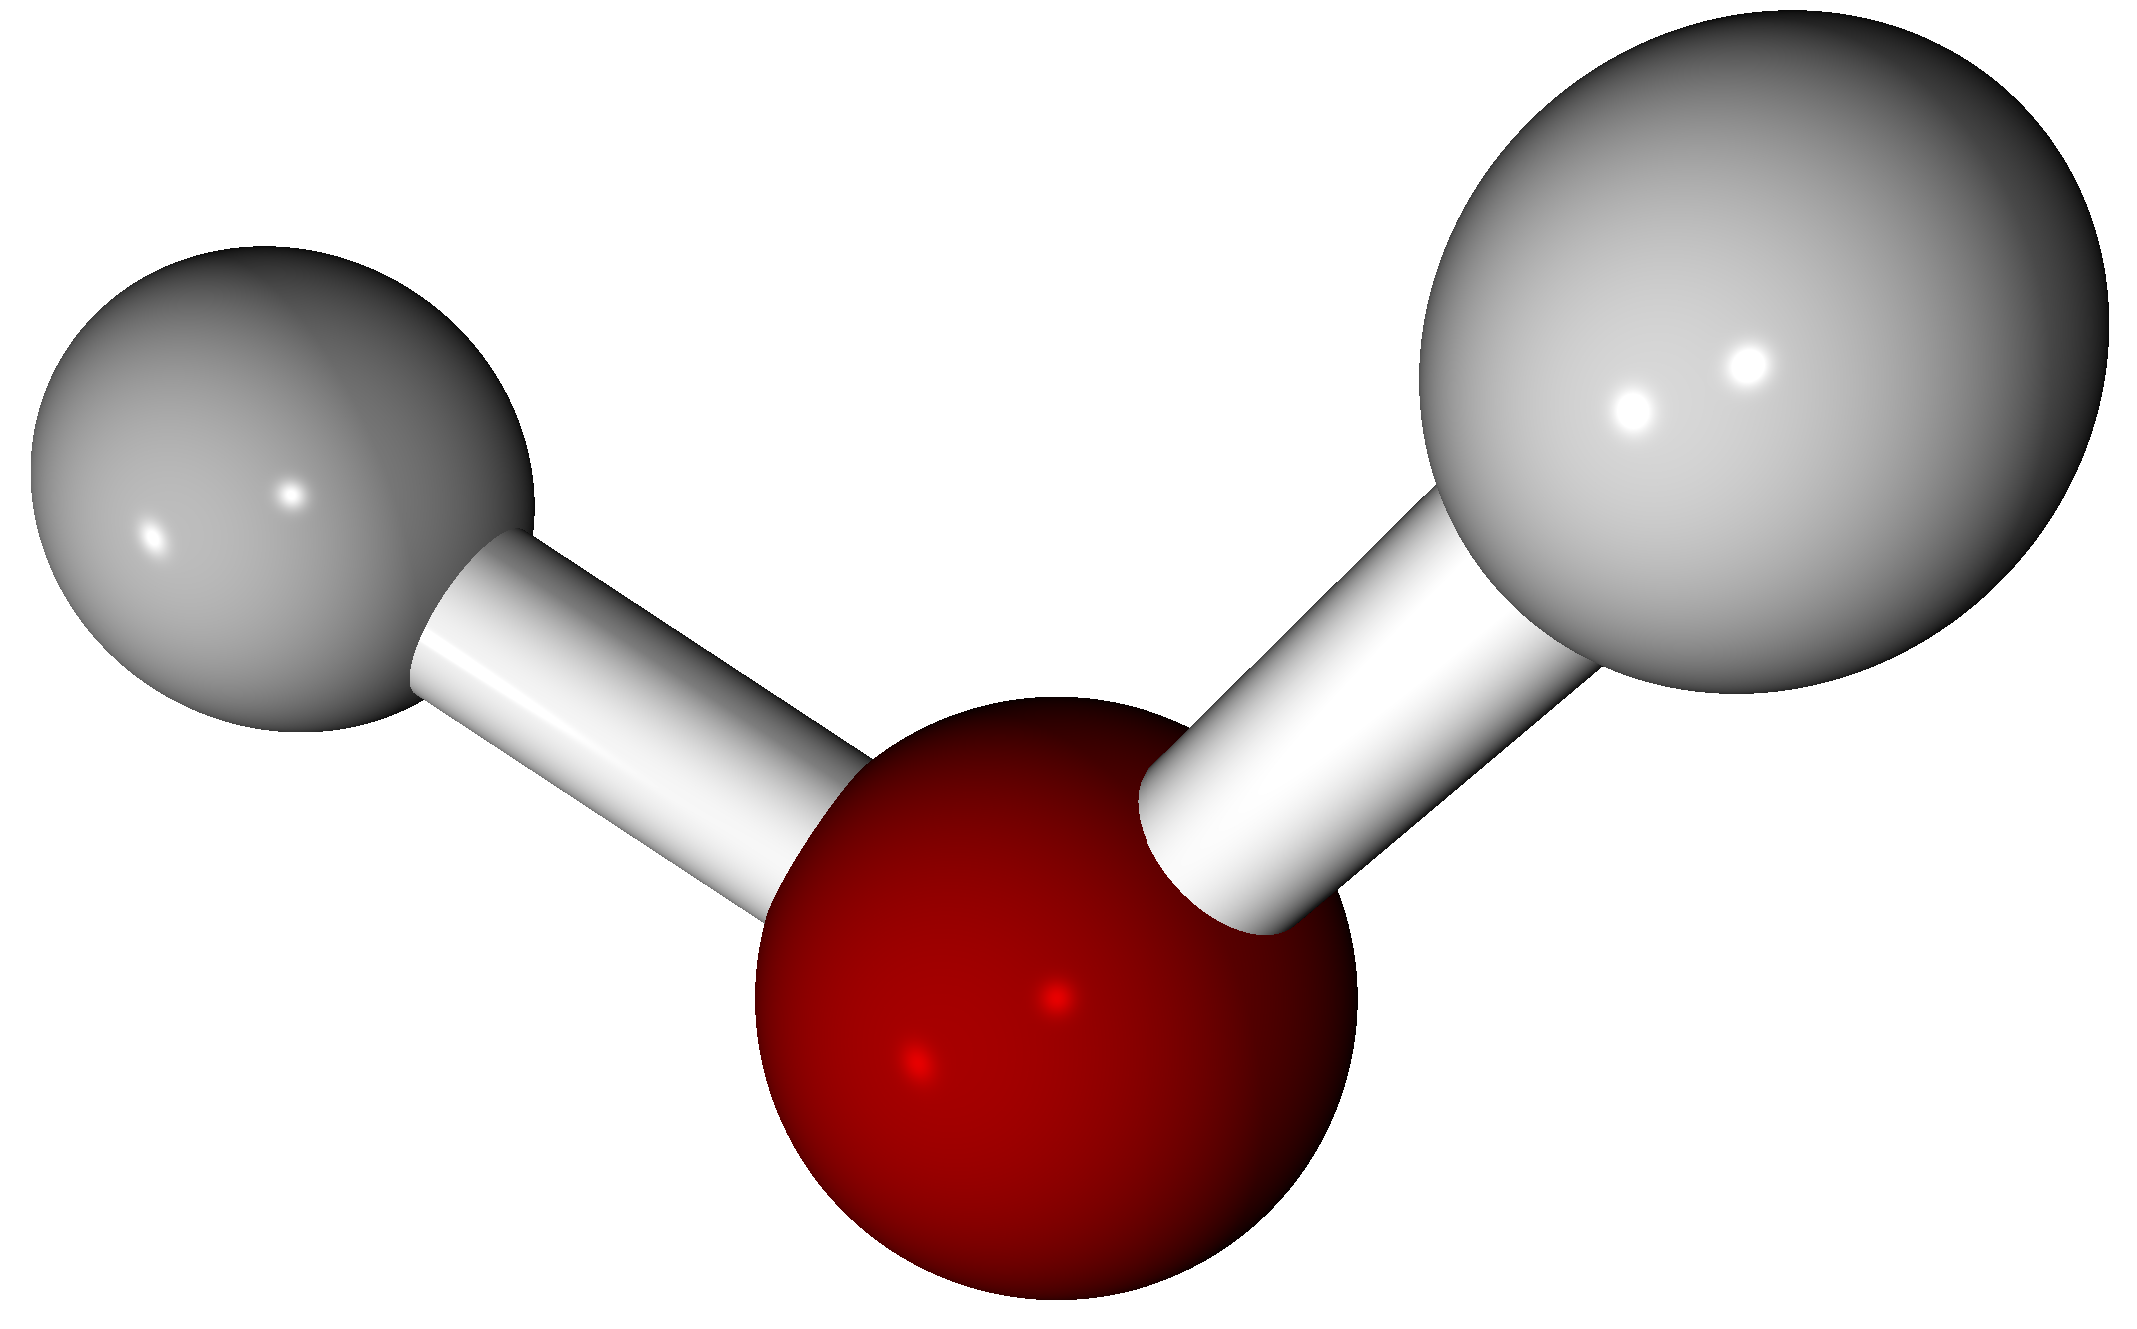
\includegraphics[width=0.5\textwidth]{final_billboard.png}
	\caption{Billboards can produce pixel perfect rendering of molecules. Here we see a water molecule being rendererd with two light sources showing specular reflection and diffuse light effects.}
	\label{fig:final_billboards}
\end{figure}

\subsection{Sphere billboards}

Each sphere is visualized as two triangles making up a square large enough to
cover all pixels the sphere needs.
To reduce the CPU workload, all 4 corner vertices of the square are placed at
the exact position of the sphere.
The radius and a vertex id is specified, so that the vertex shader can move the
4 vertices so that the plane is orthogonal to the view vector and is larger than
the cross sectional area of the sphere of interest.
This is illustrated in figure \ref{fig:billboards}.

\begin{figure}
	\centering
	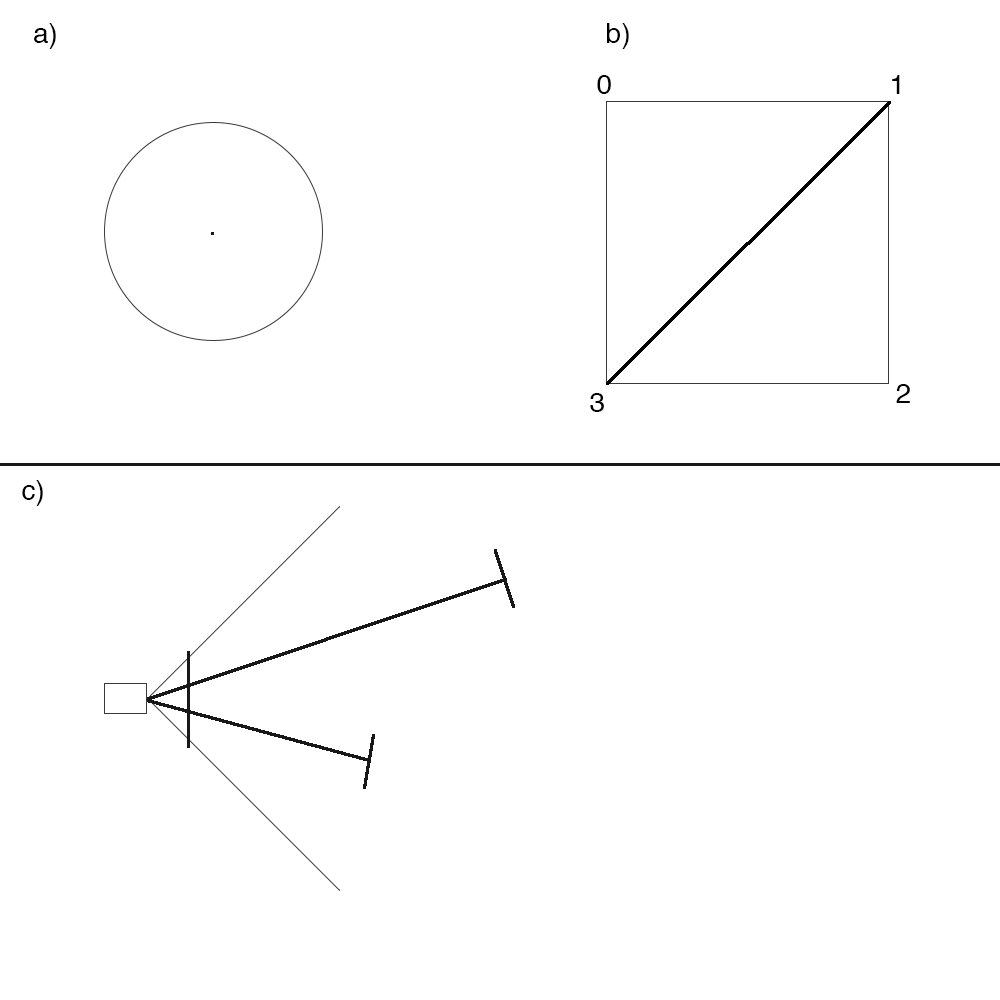
\includegraphics[width=0.5\textwidth]{spherebillboards.png}
	\caption{Illustration of billboards. The circles are shown in the figure to show our target rendering. a) all 4 vertices are at the center of the sphere. b) the vertex shader moves each vertex so that the plane covers a larger cross sectional area than the sphere. c) the orientation of the plane is such that the normal vector of the plane is parallel to the view vector. }
	\label{fig:billboards}
\end{figure}

\subsection{Cylinder billboards}
%
% TODO should we use the other terminology here rather than billboards, something about imposter visualization?
To render bonds in the molecular structure, we have implemented a method that
visualizes realistic cylinder shapes with billboards.
Cylinders are more complicated to visualize with billboards because they have a
more complex geometry.
While spheres obviously are spherically symmetric and can be rendered the same
way regardless of viewing angle, we need to take this into account when
rendering cylinders.
Furhter, the bonds need to intersect with the sphere surface in a way that
needs to be handled by the cylinder rendering technique.

The basic principle is however the same as for the spheres.
We define the vertices needed on the CPU with the same position and add the
necessary information about the cylinder to the vertex attributes.
This information is then used in the vertex shader to draw the triangles of
the billboard.
Finally, ray tracing is used to draw the final cylinder shape based on top
of this billboard.

% TODO mention issue with end caps if this is relevant for the overlapping parts

% TODO explain the details about billboard rendering?

\section{Case study (Anders)}
% Rerun on large dataset

\begin{figure}
	\centering
	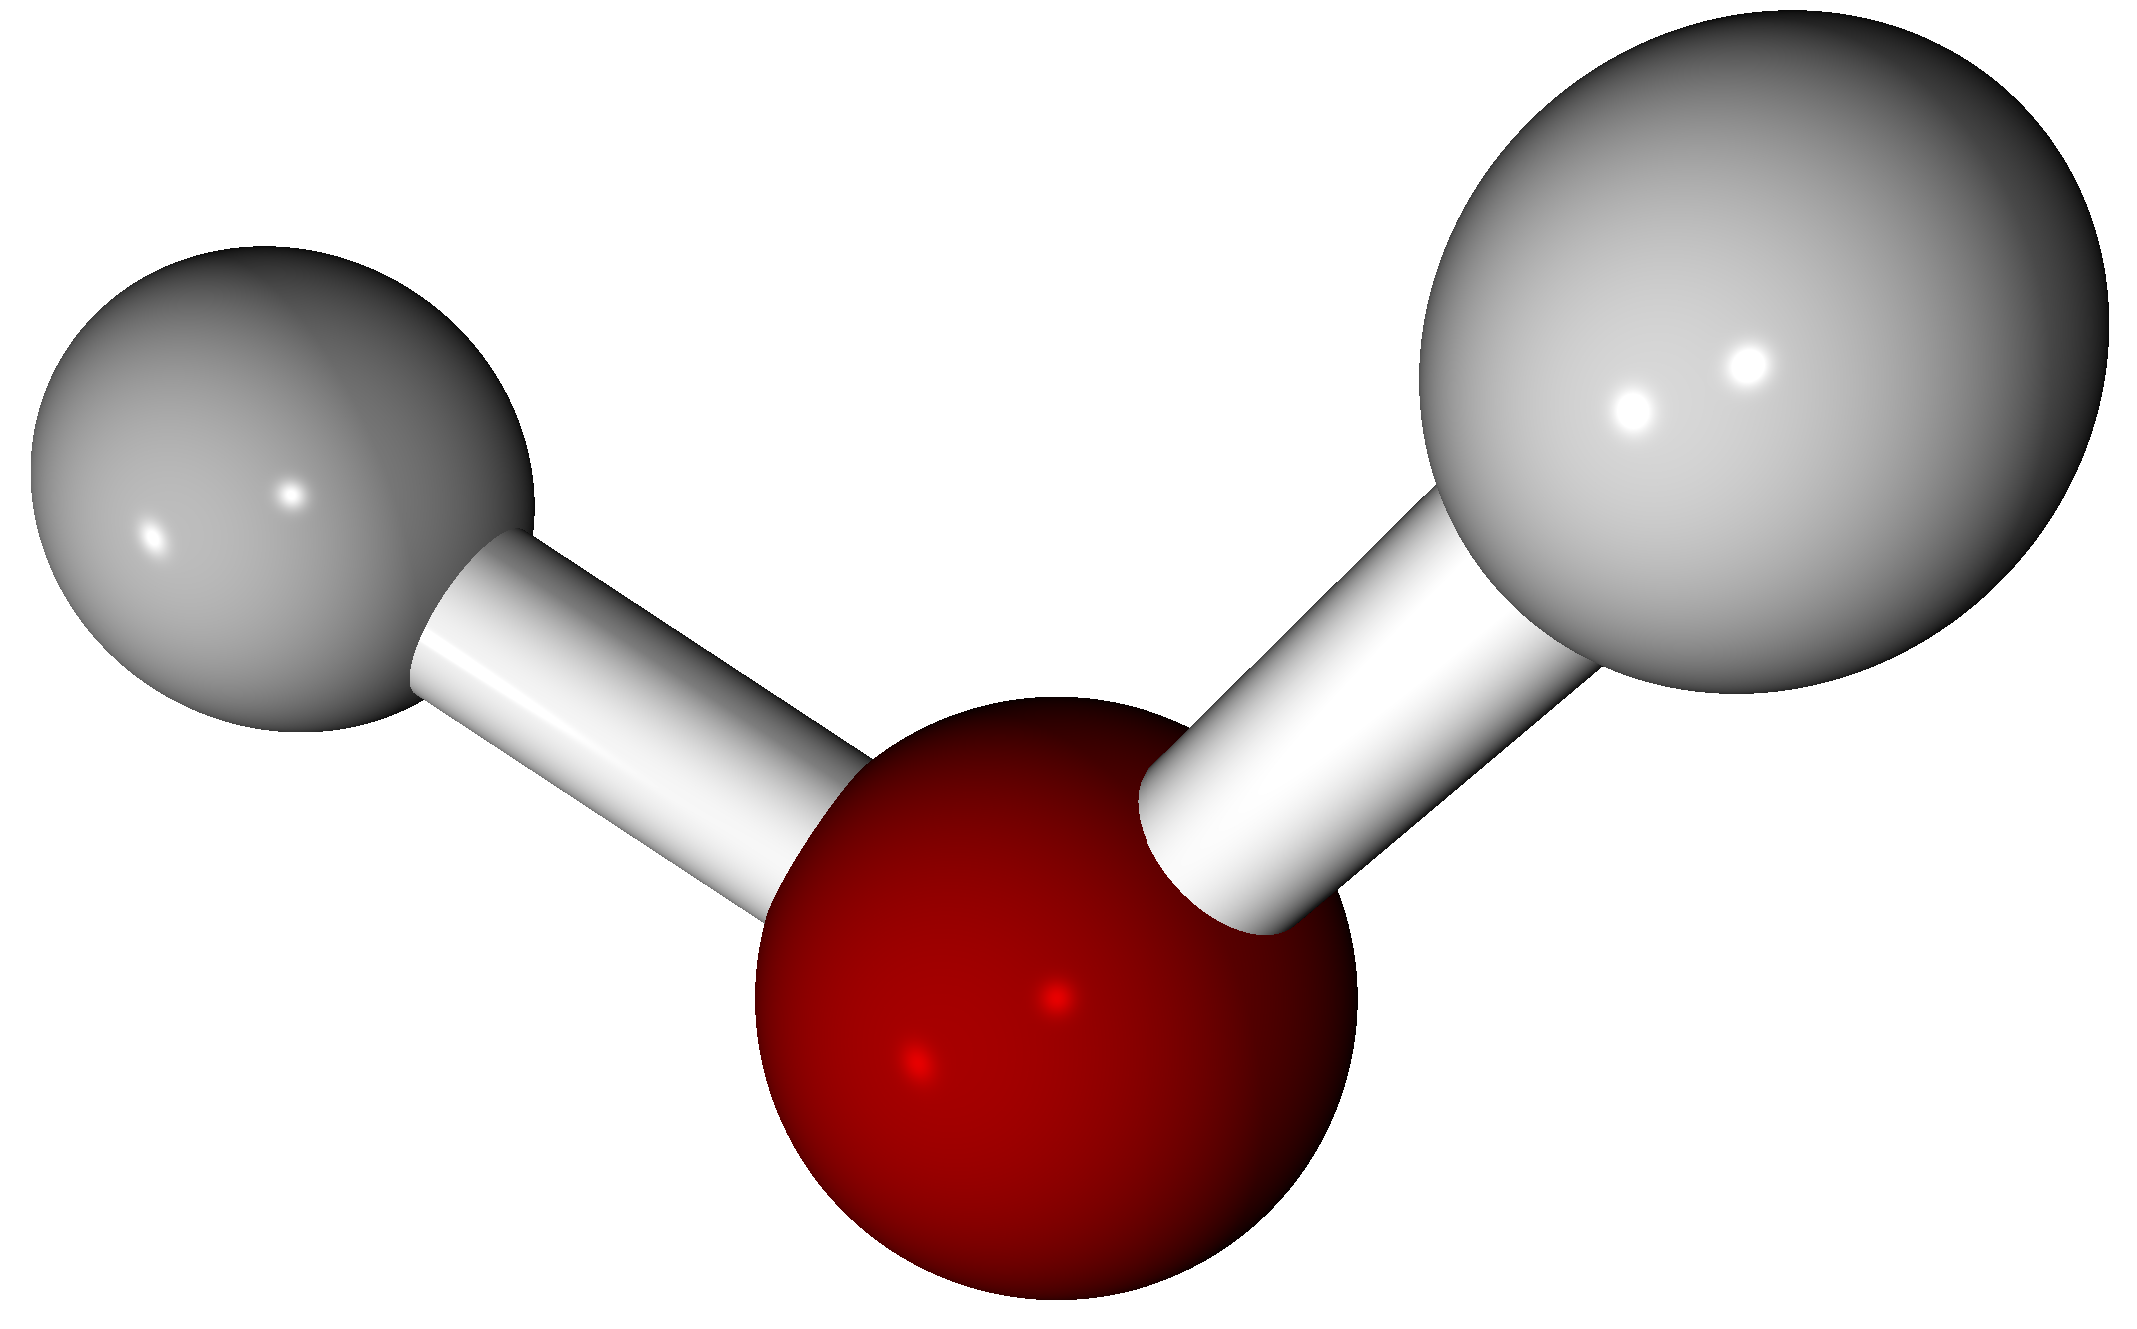
\includegraphics[width=0.5\textwidth]{final_billboard.png}
	\caption{Case study result}
	\label{fig:gui}
\end{figure}

\section{Conclusion}
%
We have presented Atomify, a software for live visualization of molecular
dynamics simulations in LAMMPS.
Atomify simplifies the workflow of researchers by combining script development,
analysis and visualization in an intuitive user interface.
The software can also be used to improve training of students using LAMMPS by
providing immediate, visual feedback to script changes.

\subsection{Future work}
Atomify is far from finished.\\
A web version of Atomify is in development using WebGL and Emscripten. \\
Geometry shaders \\
Improved script editor with auto completion \\
Moltemplate interface \\

\section{Availability}

\section{Acknowledgments}

\bibliographystyle{plain}
\bibliography{Remote}

\end{document}